% Options for packages loaded elsewhere
\PassOptionsToPackage{unicode}{hyperref}
\PassOptionsToPackage{hyphens}{url}
\PassOptionsToPackage{dvipsnames,svgnames,x11names}{xcolor}
%
\documentclass[
  singlecolumn]{article}

\usepackage{amsmath,amssymb}
\usepackage{iftex}
\ifPDFTeX
  \usepackage[T1]{fontenc}
  \usepackage[utf8]{inputenc}
  \usepackage{textcomp} % provide euro and other symbols
\else % if luatex or xetex
  \usepackage{unicode-math}
  \defaultfontfeatures{Scale=MatchLowercase}
  \defaultfontfeatures[\rmfamily]{Ligatures=TeX,Scale=1}
\fi
\usepackage[]{libertinus}
\ifPDFTeX\else  
    % xetex/luatex font selection
\fi
% Use upquote if available, for straight quotes in verbatim environments
\IfFileExists{upquote.sty}{\usepackage{upquote}}{}
\IfFileExists{microtype.sty}{% use microtype if available
  \usepackage[]{microtype}
  \UseMicrotypeSet[protrusion]{basicmath} % disable protrusion for tt fonts
}{}
\makeatletter
\@ifundefined{KOMAClassName}{% if non-KOMA class
  \IfFileExists{parskip.sty}{%
    \usepackage{parskip}
  }{% else
    \setlength{\parindent}{0pt}
    \setlength{\parskip}{6pt plus 2pt minus 1pt}}
}{% if KOMA class
  \KOMAoptions{parskip=half}}
\makeatother
\usepackage{xcolor}
\usepackage[top=30mm,left=20mm,heightrounded,top=30mm, left=20mm,
heightrounded]{geometry}
\setlength{\emergencystretch}{3em} % prevent overfull lines
\setcounter{secnumdepth}{-\maxdimen} % remove section numbering
% Make \paragraph and \subparagraph free-standing
\ifx\paragraph\undefined\else
  \let\oldparagraph\paragraph
  \renewcommand{\paragraph}[1]{\oldparagraph{#1}\mbox{}}
\fi
\ifx\subparagraph\undefined\else
  \let\oldsubparagraph\subparagraph
  \renewcommand{\subparagraph}[1]{\oldsubparagraph{#1}\mbox{}}
\fi


\providecommand{\tightlist}{%
  \setlength{\itemsep}{0pt}\setlength{\parskip}{0pt}}\usepackage{longtable,booktabs,array}
\usepackage{calc} % for calculating minipage widths
% Correct order of tables after \paragraph or \subparagraph
\usepackage{etoolbox}
\makeatletter
\patchcmd\longtable{\par}{\if@noskipsec\mbox{}\fi\par}{}{}
\makeatother
% Allow footnotes in longtable head/foot
\IfFileExists{footnotehyper.sty}{\usepackage{footnotehyper}}{\usepackage{footnote}}
\makesavenoteenv{longtable}
\usepackage{graphicx}
\makeatletter
\def\maxwidth{\ifdim\Gin@nat@width>\linewidth\linewidth\else\Gin@nat@width\fi}
\def\maxheight{\ifdim\Gin@nat@height>\textheight\textheight\else\Gin@nat@height\fi}
\makeatother
% Scale images if necessary, so that they will not overflow the page
% margins by default, and it is still possible to overwrite the defaults
% using explicit options in \includegraphics[width, height, ...]{}
\setkeys{Gin}{width=\maxwidth,height=\maxheight,keepaspectratio}
% Set default figure placement to htbp
\makeatletter
\def\fps@figure{htbp}
\makeatother
\newlength{\cslhangindent}
\setlength{\cslhangindent}{1.5em}
\newlength{\csllabelwidth}
\setlength{\csllabelwidth}{3em}
\newlength{\cslentryspacingunit} % times entry-spacing
\setlength{\cslentryspacingunit}{\parskip}
\newenvironment{CSLReferences}[2] % #1 hanging-ident, #2 entry spacing
 {% don't indent paragraphs
  \setlength{\parindent}{0pt}
  % turn on hanging indent if param 1 is 1
  \ifodd #1
  \let\oldpar\par
  \def\par{\hangindent=\cslhangindent\oldpar}
  \fi
  % set entry spacing
  \setlength{\parskip}{#2\cslentryspacingunit}
 }%
 {}
\usepackage{calc}
\newcommand{\CSLBlock}[1]{#1\hfill\break}
\newcommand{\CSLLeftMargin}[1]{\parbox[t]{\csllabelwidth}{#1}}
\newcommand{\CSLRightInline}[1]{\parbox[t]{\linewidth - \csllabelwidth}{#1}\break}
\newcommand{\CSLIndent}[1]{\hspace{\cslhangindent}#1}

\usepackage{cancel}
\usepackage[noblocks]{authblk}
\renewcommand*{\Authsep}{, }
\renewcommand*{\Authand}{, }
\renewcommand*{\Authands}{, }
\renewcommand\Affilfont{\small}
\usepackage{cancel}
\makeatletter
\makeatother
\makeatletter
\makeatother
\makeatletter
\@ifpackageloaded{caption}{}{\usepackage{caption}}
\AtBeginDocument{%
\ifdefined\contentsname
  \renewcommand*\contentsname{Table of contents}
\else
  \newcommand\contentsname{Table of contents}
\fi
\ifdefined\listfigurename
  \renewcommand*\listfigurename{List of Figures}
\else
  \newcommand\listfigurename{List of Figures}
\fi
\ifdefined\listtablename
  \renewcommand*\listtablename{List of Tables}
\else
  \newcommand\listtablename{List of Tables}
\fi
\ifdefined\figurename
  \renewcommand*\figurename{Figure}
\else
  \newcommand\figurename{Figure}
\fi
\ifdefined\tablename
  \renewcommand*\tablename{Table}
\else
  \newcommand\tablename{Table}
\fi
}
\@ifpackageloaded{float}{}{\usepackage{float}}
\floatstyle{ruled}
\@ifundefined{c@chapter}{\newfloat{codelisting}{h}{lop}}{\newfloat{codelisting}{h}{lop}[chapter]}
\floatname{codelisting}{Listing}
\newcommand*\listoflistings{\listof{codelisting}{List of Listings}}
\makeatother
\makeatletter
\@ifpackageloaded{caption}{}{\usepackage{caption}}
\@ifpackageloaded{subcaption}{}{\usepackage{subcaption}}
\makeatother
\makeatletter
\@ifpackageloaded{tcolorbox}{}{\usepackage[skins,breakable]{tcolorbox}}
\makeatother
\makeatletter
\@ifundefined{shadecolor}{\definecolor{shadecolor}{rgb}{.97, .97, .97}}
\makeatother
\makeatletter
\makeatother
\makeatletter
\makeatother
\ifLuaTeX
  \usepackage{selnolig}  % disable illegal ligatures
\fi
\IfFileExists{bookmark.sty}{\usepackage{bookmark}}{\usepackage{hyperref}}
\IfFileExists{xurl.sty}{\usepackage{xurl}}{} % add URL line breaks if available
\urlstyle{same} % disable monospaced font for URLs
\hypersetup{
  pdftitle={Causal Inference in Environmental Psychology: Through The Looking Glass of Counterfactual Data Science},
  pdfkeywords={DAGS, Causal
Inference, Confounding, History, Psychology, Panel},
  colorlinks=true,
  linkcolor={blue},
  filecolor={Maroon},
  citecolor={Blue},
  urlcolor={Blue},
  pdfcreator={LaTeX via pandoc}}

\title{Causal Inference in Environmental Psychology: Through The Looking
Glass of Counterfactual Data Science}


  \author{Donald W Hine}
            \affil{%
                  University of Canterbury, School of Psychology, Speech
                  and Hearing
              }
        \author{Joseph A. Bulbulia}
            \affil{%
                  Victoria University of Wellington, New Zealand, School
                  of Psychology, Centre for Applied Cross-Cultural
                  Research
              }
      
\date{2023-08-04}
\begin{document}
\maketitle
\begin{abstract}
Quantifying causal effects from observational data presents substantial
challenges for environmental psychologists because the correlations
obtained from observational settings are misleading causal guides.
However, recent progress in methods for causal inference brings hope for
transforming observational data into causal understanding. To clarify
the assumptions under which we may obtain causal understanding from
observational data, we provide an accessible introduction to the
potential outcomes framework of causal inference. To help researchers
better identify causation, we explain within this framework of
assumptions how to use causal Directed Acyclic Graphs (DAGs). We
conclude with practical guidelines for data collection and modelling,
reviewing ``tips'' and ``common pitfalls.'' This chapter will interest
environmental psychologists, and indeed any human scientist, who always
wanted to learn about causal inference but never thought they could.
\end{abstract}
\ifdefined\Shaded\renewenvironment{Shaded}{\begin{tcolorbox}[boxrule=0pt, frame hidden, enhanced, interior hidden, borderline west={3pt}{0pt}{shadecolor}, breakable, sharp corners]}{\end{tcolorbox}}\fi

\hypertarget{introduction}{%
\subsection{Introduction}\label{introduction}}

Correlation does not imply causation. However, quantifying a causal
effect requires drawing inferences from correlations present in the
data. It can be no other way because statistical models produce measures
of association, i.e., correlations. And to quantify effects we must
apply statistical models.

In experimental settings, quantitative causal inferences from
associational models is made possible through randomisation, controlled
interventions, and chronologically ordered data collection.

By contrast, in observational settings, the data researchers collect are
not the products of randomisation and control. Moreover, observational
researchers are often limited to cross-sectional data, which lack
temporal order. In observational settings, then, credible causal
inference from correlations can be, at best, indirect. The problems of
inferring causation in observational settings are widely known. However,
many observational researchers persist in using hedging causal language
to reporting their results, offering cautious policy recommendations
couched in words such as ``might'' and ``suggests''
(\protect\hyperlink{ref-bulbulia2022}{Bulbulia 2022}) However, because
causal association can easily run in the opposite direction of manifest
associations, every intention to report a observational correlations as
suggesting causation is more safely presumed guilty unless demonstrated
otherwise.

Are there any settings in which we might we obtain valid causal
inferences from observational data? If so, by which pathways might we
pursue such inferences?

Environmental psychologists have strong motivations to ask these
questions. Among the most compelling is an interest in understanding the
probable effects of interventions on environmental attitudes and
behaviours, which is essential for offering effective policy advice.
Moreover, although randomised experiments can sometimes afford causal
understanding, experimental studies are typically too expensive to
perform at scale. Designing and implementing interventions and then
tracking their effects over long periods are typically infeasible, and
often decisions cannot wait. Experimental control often comes at the
price of ecological validity, limiting applications. For these reasons,
the bandwidth of psychologically interesting and practically relevant
questions that experiments may address is limited. By contrast,
observational data is abundant. If we could obtain causal insights from
observational data, the state of knowledge in environmental psychology
would be greatly accelerated and the field would be better equipped to
offer advice.

Considerable progress in the methods for estimating causation from
observational data during the past twenty years offer reasons for hope
(\protect\hyperlink{ref-vanderweele2015}{VanderWeele 2015}). Although
most of this progress has occurred outside of psychology, psychological
scientists are growing increasingly interested in such methods
(\protect\hyperlink{ref-mcelreath2020}{McElreath 2020};
\protect\hyperlink{ref-rohrer2018}{Rohrer 2018}). Efforts to unite
methods for causal inference with environmental psychology, then, would
appear both promising and timely.

We believe that rate of progress in the uptake of causal inference in
environmental psychology (and in psychological science more broadly)
will turn on how rapidly researchers understand the theoretical basis on
which methods for causal inference rely. The theoretical basis of causal
effect estimation is vital because to obtain causal effect estimates
from observational data relies on assumptions. Put differently, before
researchers apply statistical methods to data, they must devote
considerable attention to planning and design than is their custom.
Whether the assumptions required for causal inference are credibly met
will typically require the input of experts familiar with the questions
at hand. In some cases the data allow reasoned guesses about whether
assumptions have been satisfied. However such cases are the exception
are rare. That causal inference relies on untestable assumptions invites
many risks. On the one hand, if we persist in demanding verification
from data researchers obtained from conventional thresholds they risk
missing causal inferences that are supported by reasonable assumptions.
On the other hand, researchers might be tempted to admit implausible
assumptions without warrant. This latter risk is particularly worrying
in those social sciences where publication biases favour results. Too
few journals are interested in studies that report uncertainty, or that
describe why results cannot be obtained from the data to hand. We
believe that to accelerate progress in environmental psychology, and in
the human sciences more generally, the theoretical foundations of causal
inference must be accessible. The assumptions that underpin causal
inference must be explained in a way that builds clear intuitions about
the underlying problem each assumption addresses. Researchers must
understand how these intuitions flow on to the tasks of data collection
and data organisation. For causal inference to bring about the
scientific transformation, each practical step from assumption to data
collection must also be grounded in solid intuitions. Because the
theoretical foundations of causal inference remain unfamilar and opaque
to most psychological scientists, including those with strong
backgrounds in statistical modelling, we believe that a gentle
introduction focussed on developing the necessary intuitions and rigour
habits may be useful.

Here, then, we present an introduction of the ``potential outcomes''
framework of causal inference, also known as the ``counterfactual''
framework for causal inference
(\protect\hyperlink{ref-hernan2023}{Hernan and Robins 2023})).

\textbf{Part 1} introduces the \emph{the three fundamental assumptions}
of causal inference. Here develop causal intuitions by anchoring them in
the framework of randomised experiments, which will be familiar to most
readers of this chapter. We shall discover that the building intuitions
for causal inference from an understanding of experiments greatly
demystify the assumptions on which causal inference relies and offers
clear directives for data collection. Surprisingly, perhaps, this
discussion will bring new theoretical understand of experiments that may
be helpful to improving their designs.

\textbf{Part 2} introduces Directed Acyclic Graphs (DAGs) -- or causal
diagrams -- as powerful tools for investigating causal assumptions in
observational settings, or in randomised experimental setting with
repeated measures. We shall discover that the functionality of causal
diagrams rests on three rules, and that these three rules in turn rest
on a robust system of mathematical proofs. The basis of causal diagrams
in mathematical proves should inspire confidence. The relative ease with
which causal diagrams can be constructed in the absence of mathematical
formalism makes causal diagrams accessible. Yet we will learn that
causal diagrams only make sense in relation to the framework of
assumptions described in Part 1. Lacking a firm grasp of these
assumptions, the application of causal diagrams to causal questions is
perilous. We offer strategies for constructing causal diagrams that will
help reserach use them safely and effectively, both in research design
and modelling.

\textbf{Part 3} Briefly reviews actionable directives for data
collection and modelling within environmental psychology and related
fields. This advice will be useful human scientists who seek
quantitative understanding about the probable effects of interventions
on environmental attitudes and behaviours.

\hypertarget{part-1.-an-introduction-to-the-potential-outcomes-framework-of-causal-inference.}{%
\subsection{Part 1. An introduction to the potential outcomes framework
of causal
inference.}\label{part-1.-an-introduction-to-the-potential-outcomes-framework-of-causal-inference.}}

The content provided is both accurate and well-articulated, with a few
minor exceptions. The below edits clarify some of the language and fix
minor errors:

\hypertarget{part-1-an-introduction-to-the-potential-outcomes-framework-of-causal-inference}{%
\subsection{Part 1: An Introduction to the Potential Outcomes Framework
of Causal
Inference}\label{part-1-an-introduction-to-the-potential-outcomes-framework-of-causal-inference}}

\hypertarget{step-1-understand-that-we-assess-the-relationships-of-cause-and-effect-by-contrasting-the-outcomes-of-interventions}{%
\subsubsection{Step 1: Understand that we assess the relationships of
cause and effect by contrasting the outcomes of
interventions}\label{step-1-understand-that-we-assess-the-relationships-of-cause-and-effect-by-contrasting-the-outcomes-of-interventions}}

Suppose we are interested in well-being. Given this interest, we might
be curious about understanding the factors that influence it. One such
factor could be the accessibility of urban green spaces {[}CITE{]}. That
is, living closer to abundant green spaces may enhance well-being
compared to living in an environment devoid of such abundance. How might
we obtain a quantitative causal understanding?

First, we define a `cause'. In a setting of causal inference, a cause is
equivalent to an ``intervention'' or ``exposure'' or ``treatment.''

Second, we define an ``effect.'' In a setting of causal inference, an
effect is the outcome of the intervention. To quantitatively understand
the effect of a cause or intervention, we state a contrast of outcomes
under two interventions at some scale of measurement. For example, the
effect of abundant green spaces for individual \(i\) may be expressed
as:

\[
\text{Well-being effect of abundant greenspace}_{i} = \text{Well-being of abundant green space}_i - \text{Well-being of no abundant green space}_i
\]

We could also express this contrast on a ratio scale:

\[
\text{Well-being effect of abundant greenspace}_i = \frac{\text{Well-being of abundant green space}_i}{\text{Well-being of no abundant green space}_i}
\]

\hypertarget{step-1.1-quantifying-a-causal-effect-demands-a-contrast-of-interventions}{%
\paragraph{\texorpdfstring{\textbf{Step 1.1: Quantifying a causal effect
demands a contrast of
interventions}}{Step 1.1: Quantifying a causal effect demands a contrast of interventions}}\label{step-1.1-quantifying-a-causal-effect-demands-a-contrast-of-interventions}}

The concept of causal effect requires at least two potential
interventions. Comparing outcomes under these different interventions
provides insight into causation. For instance, contrasting an
intervention against its absence always yields zero contrast in effects,
represented mathematically as:

\[
\text{Effect of abundant greenspace} = \text{Effect of abundant green space} - \text{Effect of abundant green space} = 0
\]

The contrast of potential outcomes under different interventions offers
evidence for causation when the contrast does not equal zero:

\[
\text{Causal effect of Do X} = \text{Causal effect of Do  X} - \text{Causal Effect of Do Not X} \neq 0
\]

Depending on the residual quantity, we can determine whether the effect
is positive, negative, or null.

\hypertarget{step-2-understand-that-causation-occurs-in-time}{%
\subsubsection{Step 2: Understand that causation occurs in
time}\label{step-2-understand-that-causation-occurs-in-time}}

Causes are related to effects by time. We may say, ``each effect is
borne of a cause.'' That is, at the scale of the the universe that
people occupy, effects cannot precede their. Although intuitive, this
concept is often overlooked in psychological science. For instance,
causation requires that we assume:

\[
\text{cause} \to \text{effect}
\]

However, when we work with cross-sectional data, we cannot generally
rule out:

\[
\text{labelled effect} \to \text{labelled cause}
\]

Therefore, we should be wary of cross-sectional data for causal
inference.

\hypertarget{step-3-understand-that-causal-inference-is-requires-contrasting-potential-or-counterfactual-outcomes-that-are-never-fully-observed.}{%
\subsubsection{Step 3: Understand that causal inference is requires
contrasting ``potential'' (or ``counterfactual'') outcomes that are
never fully
observed.}\label{step-3-understand-that-causal-inference-is-requires-contrasting-potential-or-counterfactual-outcomes-that-are-never-fully-observed.}}

\hypertarget{proof-by-contradiction-that-individual-causal-effects-are-not-observed.}{%
\paragraph{\texorpdfstring{\textbf{Proof by contradiction that
individual causal effects are not
observed.}}{Proof by contradiction that individual causal effects are not observed.}}\label{proof-by-contradiction-that-individual-causal-effects-are-not-observed.}}

Assume that individual causal effects can be fully observed. This
implies that for an individual, we can observe both the effect of taking
a decision (exposure to abundant green space) and not taking the
decision (no living with abundant green space) simultaneously. However,
by definition, an individual can only exist in one state at a time ---
either one has green space access or they do not -- we cannot have both.

This contradicts our initial assumption, leading us to conclude that
individual causal effects can never be fully observed.

Another proof is as follows:

\hypertarget{direct-proof-individual-causal-effects-are-not-observed.}{%
\paragraph{\texorpdfstring{\textbf{Direct proof individual causal
effects are not
observed.}}{Direct proof individual causal effects are not observed.}}\label{direct-proof-individual-causal-effects-are-not-observed.}}

Consider a scenario where the causal effect for an individual is
understood as the difference in outcomes under two distinct scenarios
--- one where a decision is enacted (for example, enjoying green space)
and one where it is not (devoid of green space).

However, for any individual in a particular moment, only one of these
circumstances can occur ---- the individual either embraces green space
or they do not. We can only observe the outcome corresponding to the
actual decision made, but we cannot observe the outcome for the
counterfactual scenario (the decision not enacted).

In the language of causal inference, individual causal effects encounter
the ``fundamental problem of causal inference''
(\protect\hyperlink{ref-holland1986}{Holland 1986};
\protect\hyperlink{ref-rubin1976}{Rubin 1976}). That is, individual
causal effects are necessarily only partially observed.

\hypertarget{step-3.1-the-implication-causal-inference-requires-solving-a-special-and-peculiar-missing-data-problem}{%
\paragraph{\texorpdfstring{\textbf{Step 3.1: The implication: causal
inference requires solving a special and peculiar missing data
problem}}{Step 3.1: The implication: causal inference requires solving a special and peculiar missing data problem}}\label{step-3.1-the-implication-causal-inference-requires-solving-a-special-and-peculiar-missing-data-problem}}

If we are to quantify causal effects, our challenge is to bridge the gap
between the observable world and the inherently unobservable world.
Causal inference is a missing data problem (Westreich \emph{et al.}
(\protect\hyperlink{ref-westreich2015}{2015}); Edwards \emph{et al.}
(\protect\hyperlink{ref-edwards2015}{2015}))

\hypertarget{step-4-understand-that-the-problem-of-missing-counterfactual-is-easier-to-solve-when-the-target-of-inference-is-the-average-or-marginal-causal-effect-obtained-from-an-experiment}{%
\subsubsection{Step 4: Understand that the problem of missing
counterfactual is easier to solve when the target of inference is the
average (or marginal) causal effect obtained from an
experiment}\label{step-4-understand-that-the-problem-of-missing-counterfactual-is-easier-to-solve-when-the-target-of-inference-is-the-average-or-marginal-causal-effect-obtained-from-an-experiment}}

The average causal effect represents the difference in average outcomes
of a population under two distinct treatment conditions. In formal
terms, the average causal effect of a treatment (A) on an outcome (Y)
can be defined as follows:

\[
\text{Average Causal Effect} = \mathbb{E}[Y(A = 1)] - \mathbb{E}[Y(A = 0)]
\]

where \(\mathbb{E}[Y(A = a)]\) denotes the expected value of the outcome
under treatment condition \(A = a\). Here, \(A = 1\) indicates the
presence of the treatment, while \(A = 0\) represents its absence.

\hypertarget{step-4.1-understand-that-the-problem-of-missing-counterfactual-outcomes-remains-for-average-treatment-effects.}{%
\paragraph{Step 4.1 Understand that the problem of missing
counterfactual outcomes remains for average treatment
effects.}\label{step-4.1-understand-that-the-problem-of-missing-counterfactual-outcomes-remains-for-average-treatment-effects.}}

Thatt the problem of missing counterfactuals remains for average
treatment effects becomes evident when we consider a scenario involving
two contrasting states: the presence of treatment (\(A = 1\)) and the
absence of treatment (\(A = 0\)).

If an individual is subjected to treatment, we observe the outcome
\(Y_{\text{observed}_i}|A_i = 1\), but miss the counterfactual outcome
\(Y(A_i = 0)\), i.e., the outcome if the individual had not received the
treatment.

Similarly, if the treatment is not administered, we observe
\(Y_{\text{observed}_i}|A_i = 0\), but miss the counterfactual outcome
\(Y(A_i = 1)\).

Thus, for each individual, only one of the potential outcomes is
observed, and the other one is missing. The challenge is that we cannot
compute the individual causal effect, \(Y(A_i = 1) - Y(A_i = 0)\),
because we only observe one of the two terms for each individual.

To compute the average causal effect over a population, we should
ideally sum these individual causal effects and divide by the population
size:

\[
\text{Average Causal Effect} = \frac{1}{N}\sum_{i=1}^{N} [Y(A_i = 1) - Y(A_i = 0)]
\]

However, as we only observe one term of the subtracted pair for each
individual, we cannot calculate this sum directly. We again encounter
the fundamental problem in causal inference when calculate average
causal effects: the problem of individual-level missing counterfactuals
persists ``under the hood'' of each intervention that we seek to
compare.

\hypertarget{step-4.2-understand-how-experiments-satisfy-assumptions-need-to-impute-missing-responses-that-are-needed-to-obtain-average-treatment-effects}{%
\paragraph{Step 4.2 Understand how experiments satisfy assumptions need
to impute missing responses that are needed to obtain average treatment
effects}\label{step-4.2-understand-how-experiments-satisfy-assumptions-need-to-impute-missing-responses-that-are-needed-to-obtain-average-treatment-effects}}

Randomised experiments are designed to impute missing counterfactuals
that are necessary to calculate average treatment effects by random
treatment assignment. To build intuitions that enable understanding for
how experiments recover missing counterfactuls, consider their defining
features.

\hypertarget{step-4.3.-understand-the-principle-of-randomisation}{%
\paragraph{\texorpdfstring{\textbf{Step 4.3. Understand the principle of
randomisation}}{Step 4.3. Understand the principle of randomisation}}\label{step-4.3.-understand-the-principle-of-randomisation}}

In a random experiment, each participant has an equal chance of being in
either the treatment or the control group. This concept can be
formulated:

\[
\text{Randomisation} = \text{Equal Probability of Assignment to Groups}
\]

\hypertarget{step-4.5.-define-experiment-with-reference-measurement-of-interventions}{%
\subparagraph{\texorpdfstring{\textbf{Step 4.5. Define experiment with
reference measurement of
interventions}}{Step 4.5. Define experiment with reference measurement of interventions}}\label{step-4.5.-define-experiment-with-reference-measurement-of-interventions}}

An experiment is an event in which an experimenter (or group of
experimenters) applies different treatments to another group by virtue
of randomised assignment. Thus, an experiment consists is constituted as
follows:

\[
\text{Experiment} = \text{Controlled Application of Interventions + Measurement of Outcome}
\]

\hypertarget{step-4.6.-understand-that-experiments-align-potential-outcomes-with-observed-outcomes-by-satisfying-a-causal-consistency-assumption}{%
\subparagraph{\texorpdfstring{\textbf{Step 4.6. Understand that
experiments align potential outcomes with observed outcomes by
satisfying a causal consistency
assumption}}{Step 4.6. Understand that experiments align potential outcomes with observed outcomes by satisfying a causal consistency assumption}}\label{step-4.6.-understand-that-experiments-align-potential-outcomes-with-observed-outcomes-by-satisfying-a-causal-consistency-assumption}}

Causal consistency is the assumption that the potential outcome under an
intervention level is equivalent to the observed outcome when that
intervention is applied.

In the context of an experiment, observed outcomes may be credibly
mapped one-to-one with potential outcomes.

Recall that \(Y(a)\) denotes the potential outcome under treatment level
\(A = a\). Let \(\delta_{ate}\)\} denote the average causal effect on
the difference scale. The target of causal inference for the average
causal effect of a treatment is thus

\[
\delta_{ate} = E[Y(1)] - E[Y(0)]
\]

This represents the contrast in average outcome under treatment and
average outcome without treatment.

\hypertarget{step-4.7.-understand-that-experiments-satisfy-a-causal-consistency-assumption-thus-recovering-half-of-the-potential-outcomes-needed-for-estimating-the-ate}{%
\subparagraph{\texorpdfstring{\textbf{Step 4.7. Understand that
experiments satisfy a causal consistency assumption, thus recovering
half of the potential outcomes needed for estimating the
ATE}}{Step 4.7. Understand that experiments satisfy a causal consistency assumption, thus recovering half of the potential outcomes needed for estimating the ATE}}\label{step-4.7.-understand-that-experiments-satisfy-a-causal-consistency-assumption-thus-recovering-half-of-the-potential-outcomes-needed-for-estimating-the-ate}}

In an experiment, when a treatment (\(A = 1\)) is applied, we assume the
observed outcome aligns with the potential outcome under treatment:

\[
(Y_{\text{observed}_i}|A_i = 1) = Y_i(1)
\]

And similarly, when no treatment (\(A = 0\)) is administered, the
observed outcome corresponds to the potential outcome without treatment:

\[
(Y_{\text{observed}_i}|A_i = 0) = Y_i(0)
\]

In other words, if an individual is assigned to the treatment group
(\(A_i = 1\)), then the observed outcome corresponds to the potential
outcome under treatment (\(Y_i(a_i = 1)\)). Similarly, for those in the
control group (\(A_i = 0\)), the observed outcomes correspond to the
potential outcomes under no treatment (\(Y_i(a_i = 0)\)).

Thus, causal consistency allows us to infer the potential outcomes
corresponding to the actual treatment each individual receives.

\hypertarget{step-4.8.-understand-that-experiments-satisfy-a-causal-consistency-assumption-thus-recovering-half-of-the-potential-outcomes-needed-for-estimating-the-ate}{%
\paragraph{\texorpdfstring{\textbf{Step 4.8. Understand that experiments
satisfy a causal consistency assumption, thus recovering half of the
potential outcomes needed for estimating the
ATE}*}{Step 4.8. Understand that experiments satisfy a causal consistency assumption, thus recovering half of the potential outcomes needed for estimating the ATE*}}\label{step-4.8.-understand-that-experiments-satisfy-a-causal-consistency-assumption-thus-recovering-half-of-the-potential-outcomes-needed-for-estimating-the-ate}}

Exchangeability is a statistical concept implying that, in expectation,
the distribution of potential outcomes is the same under different
treatment conditions, regardless of the treatment assignment. This is to
say, if we were able to have God-like access to all the potential
outcomes, we would not expect systematic differences between those
assigned to treatment and those assigned to control.

This assumption is typically ensured in experimental designs by
\textbf{by randomisation}. Random assignment to treatment ensures that
all observed and unobserved characteristics are, on average, evenly
distributed between treatment and control groups. Thus, any difference
in the observed outcomes between these groups can be attributed to the
treatment effect, rather than to systematic differences in the groups.

Thus, under the assumption of exchangeability, the observed outcomes in
the control group can be used to estimate the unobserved potential
outcomes in the treatment group and vice versa. This allows us to impute
the missing half of the potential outcomes required for ATE estimation.

\hypertarget{step-4.8.-understand-that-experiments-satisfy-a-positivity-assumption-thus-ensuring-that-the-causal-contrasts-that-we-compute-are-not-impossible.}{%
\paragraph{\texorpdfstring{\textbf{Step 4.8. Understand that experiments
satisfy a positivity assumption, thus ensuring that the causal contrasts
that we compute are not
impossible.}}{Step 4.8. Understand that experiments satisfy a positivity assumption, thus ensuring that the causal contrasts that we compute are not impossible.}}\label{step-4.8.-understand-that-experiments-satisfy-a-positivity-assumption-thus-ensuring-that-the-causal-contrasts-that-we-compute-are-not-impossible.}}

Positivity is a vital assumption for causal inference in observational
settings. However in experiments it is so obviously satisfied that the
assumption is easly overlooked. The assumption states that every unit
has a non-zero probability of receiving each level of treatment. Because
experimentalists actively intervene in the world, positivity is ensured.
Positivity esures we always have data to estimate the potential
outcomes. As such, we can compute the average causal effect. However in
observational settings, it is precisely control that is lacking. The
data that we need to assess causal effects may fail if (1) \textbf{weak
positivity} is violated: the relevant observations have not been
collected. For example if moving either to abundant greenspace or away
from abundant greenspace is exceedly rare, the data might be
insufficient to compute average causal contrast; (2) \textbf{strong
positivity} is violated: the intervention is impossible: e.g.~data are
collected in country were all green spaces have been destroyed.

\hypertarget{step-5-build-intuitions-for-how-causal-assumptions-may-be-translated-from-experimental-to-observational-settings}{%
\subsubsection{Step 5: Build intuitions for how causal assumptions may
be translated from experimental to observational
settings}\label{step-5-build-intuitions-for-how-causal-assumptions-may-be-translated-from-experimental-to-observational-settings}}

The leap from controlled experiments to observational research typically
poses challenges because outside of experiments the conditions that
satisfy consistency, exchangeability, and positivity are not
automatically satisfied.

In experiments, we have:

\[
\delta_{ate} = E[Y | do(A = 1)] - E[Y | do(A = 0)]
\]

Where \[E[Y | do(A = 1)]\] is the expected outcome if we apply the
treatment to the entire population, and \[E[Y | do(A = 0)]\] is the
expected outcome if we withhold the treatment from the entire
population. However, in observational settings, we simply have the
observed association:

\[
OA = E[Y | A = 1] - E[Y | A = 0]
\]

Next we consider the problems in equating \(0A\) with \(\delta_{ate}\)
by offering any interpretation of raw correlations in observational data
(including cautious suggestions of causality.)

\hypertarget{step-5.1.-understand-how-causal-consistency-may-fail-in-observational-settings}{%
\paragraph{\texorpdfstring{\textbf{Step 5.1. Understand how causal
consistency may fail in observational
settings}}{Step 5.1. Understand how causal consistency may fail in observational settings}}\label{step-5.1.-understand-how-causal-consistency-may-fail-in-observational-settings}}

The application of treatments in an observational setting may not be
consistent. Consider the case of moving closer to abundant green spaces.
Here, what constitutes ``moving closer to abundant green spaces'' is
rarely the same intervention across the population that moves. The
intervention might differ in the following ways:

\begin{enumerate}
\def\labelenumi{\alph{enumi}.}
\item
  Diversity in green spaces: green spaces may vary widely in terms of
  biodiversity and aesthetic appeal, hence leading to varying
  treatments, which may affect outcomes.
\item
  Availability of amenities: green spaces equipped with walking paths,
  benches, recreational, and especially cafes, create differences in the
  treatments, which may affect outcomes.
\item
  Variation in proximity: How close an individual is to a green space
  can vary, influencing access and frequency of use, again the
  treatments compared do not resemble those of controlled experiments.
\item
  Size and type of green space: the outcomes can vary depending on
  whether the green space is a park, forest, or community garden.
\end{enumerate}

When we try to define the ``treatment'' of abundant access to green
spaces it is clear that nearly every attempt to do so will fall short of
a hypothetical experiment in which a researchers intervene to
consistently control the experience.

\hypertarget{step-5.2.-understand-how-exchangeability-may-fail-in-observational-settings}{%
\paragraph{\texorpdfstring{\textbf{Step 5.2. Understand how
exchangeability may fail in observational
settings}}{Step 5.2. Understand how exchangeability may fail in observational settings}}\label{step-5.2.-understand-how-exchangeability-may-fail-in-observational-settings}}

In an observational study, it is easy to imagine that individuals in
different treatment groups are systematically different. For example,
people moving closer to green spaces may differ on several attributes,
including:

\begin{enumerate}
\def\labelenumi{\alph{enumi}.}
\item
  Socioeconomic status: Individuals from different economic strata may
  perceive and utilise green spaces differently.
\item
  Age: Younger individuals may have different outcomes from green spaces
  compared to older individuals.
\item
  Mental health status: Individuals with better mental health might be
  more inclined to move closer to green spaces.
\item
  Lifestyle preferences: Those with outdoor lifestyle preferences might
  choose to live near green spaces, but their lifestyle, not the green
  space, could be causing the effect.
\item
  Personal values: People who value sustainability may perceive greater
  benefits from living near green spaces, rendering the comparison
  groups different in ways that affect outcomes.
\item
  Social connections: Individuals with strong community ties may
  perceive more benefits from green spaces, and the distribution of such
  people might vary between conditions.
\end{enumerate}

Again there are many ways in which groups that are not randomly assigned
to the conditions we wish to compare might differ in ways that affect
observed well-being independly of access to abundant urban greenspaces.

\hypertarget{step-5.3.-understand-how-positivity-may-fail-in-observational-settings}{%
\paragraph{\texorpdfstring{\textbf{Step 5.3. Understand how positivity
may fail in observational
settings}}{Step 5.3. Understand how positivity may fail in observational settings}}\label{step-5.3.-understand-how-positivity-may-fail-in-observational-settings}}

Positivity could fail for the reasons we discussed, either because the
exposure is too rare (violating weak positivity in the data) or because
the exposure could not occur (violating strong positivity). Again,
lacking experimental control, positivity cannot be assumed without
considering contextual details. Notably, satisfaction of (weak)
positivity is the one fundamental assumption of causal inference that
can be assessed by observing the distribution of interventions in the
data. For example, if the intervention is too rare to evaluate, or is
missing within certain strata of our comparison groups, we say that weak
positivity is violated. And we should stop our study there.

\hypertarget{step-6.-build-intution-for-how-the-fundamental-assumptions-for-causal-inference-may-be-satisfied-in-observational-settings}{%
\subsubsection{Step 6. Build intution for how the fundamental
assumptions for causal inference may be satisfied in observational
settings}\label{step-6.-build-intution-for-how-the-fundamental-assumptions-for-causal-inference-may-be-satisfied-in-observational-settings}}

\hypertarget{step-6.1-understand-how-we-may-use-the-theory-of-causal-inference-under-multiple-versions-of-treatment-to-address-causal-consistency-in-observational-settings.}{%
\paragraph{\texorpdfstring{\textbf{Step 6.1 Understand how we may use
the theory of causal inference under multiple versions of treatment to
address causal consistency in observational
settings}.}{Step 6.1 Understand how we may use the theory of causal inference under multiple versions of treatment to address causal consistency in observational settings.}}\label{step-6.1-understand-how-we-may-use-the-theory-of-causal-inference-under-multiple-versions-of-treatment-to-address-causal-consistency-in-observational-settings.}}

In observational research, there are typically multiple versions of
treatment. The theory of causal inference under multiple versions of
treatment proves we can consistently estimate causal effects where the
different versions of treatment are conditionally independent of the
outcomes VanderWeele (\protect\hyperlink{ref-vanderweele2009}{2009})
(See Appendix 1 for additional discussion of the proof and its
implications.)

Let \(\coprod\) denote independence. Where there are \(K\) different
versions of treatment \(A\) and no confounding for \(K\)'s effect on
\(Y\) given measured confounders \(L\) such that

\[
Y(k) \coprod K | L
\]

Then it can be proved that causal consistency follows.According to the
theory of causal inference under multiple versions of treatment, the
measured variable \(A\) functions as a ``coarsened indicator'' for
estimating the causal effect of the multiple versions of treatment \(K\)
on \(Y(k)\) (\protect\hyperlink{ref-vanderweele2009}{VanderWeele 2009},
\protect\hyperlink{ref-vanderweele2018}{2018};
\protect\hyperlink{ref-vanderweele2013}{VanderWeele and Hernan 2013}).

In the context of green spaces, \(A\) might represent the general action
of moving closer to any green space and \(K\) represents the different
versions of this treatment. For instance, \(K\) could denote moving
closer to different types of green spaces such as parks, forests,
community gardens, or green spaces with varying amenities and features.

Here, the conditional independence implies that, given measured
confounders \(L\) (e.g.~socioeconomic status, age, personal values), the
type of green space one moves closer to (\(K\)) is independent of the
outcomes \(Y(k)\) (e.g.~mental well-being under the \(K\) conditions).
In other words, the version of green space one chooses to live near does
not affect the \(K\) potential outcomes, provided the confounders \(L\)
are properly controlled for in our statistical models.

Here, the measured variable \(A\) (moving closer to green spaces)
functions as a simplified or ``coarsened indicator'' for the causal
effect of multiple versions of the treatment \(K\) (moving closer to
different types of green spaces) on \(Y(k)\) (health outcomes). This
suggests we can estimate the causal effect of moving closer to green
spaces in general, even though this treatment consists of multiple
versions, as long as the conditions of conditional independence are
satisfied.

\hypertarget{step-6.2-understand-how-we-may-condition-on-confounders-to-address-the-assumption-of-conditional-exchangeability}{%
\subsubsection{\texorpdfstring{\textbf{Step 6.2 Understand how we may
condition on confounders to address the assumption of (conditional)
exchangeability}}{Step 6.2 Understand how we may condition on confounders to address the assumption of (conditional) exchangeability}}\label{step-6.2-understand-how-we-may-condition-on-confounders-to-address-the-assumption-of-conditional-exchangeability}}

We say that conditional exchangeability is satisfied if, after
controlling for observed covariates, the assignment of treatment is
independent of the potential outcomes under treatment. Conceptually,
assuming both causal consistency (including no interference) and
positivity are satisfied, satisfaction of the conditional
exchangeability assumption implies that if units were swapped between
treatment conditions, the distribution of potential outcomes under
different exposures would remain unchanged. This assumption is needed to
ensure a balance between exposures in confounders that might affect the
outcome. With this assumption satisfied, the counterfactual observations
derived from the consistency and positivity assumptions can be viewed as
randomly assigned to the exposure conditions under which they were
observed. In effect (so to speak), satisfying the conditional
exchangeability assumption is an attempt to simulate experimentally
controlled randomisation with observational data.

Let \(L\) to be the set of measured covariates required to ensure
conditional independence. Let \(\coprod\) denote independence. We
express the exchangeability of counterfactual outcomes conditional on
measured covariates \(L\) as

\[
Y(a) \coprod  A|L
\]

Where the exchangeability assumption holds, along with the consistency
and positivity assumptions, we may express the average treatment effect
(ATE) on the difference scale

\[
\delta_{ATE}  = \mathbb{E}[Y(a^*)|L = l] - \mathbb{E}[Y(a)|L = l]
\]

Satisfaction of this assumption allows us to approximate a randomised
experiment with observational data.

Considering once again causal inference for the effect on metnal
well-being of moving closer to green spaces, \(A\) represents this move
(the treatment), while \(Y(a)\) denotes the potential outcomes of move
on well-being.

\(L\) denotes the set of measured confounders that might influence both
the decision to move closer to a green space and the potential outcomes
(or that may be an effect of such factors). Again, these confounders
might include factors suchas socioeconomic status, age, mental health
status, lifestyle preferences, personal values, social connections,
occupational demands, family circumstances, economic factors.

If the set of observed covariates is sufficient to measure all the
factors that could explain away the association of treatment and
outcome, we may say that the conditional exchangeability assumption is
satisfied. Typically this assumption cannot be tested by observational
data. For this reason, it is important to perform sensitivity analyses
to evaluate how much unmeasured confounding would be required to explain
away any observed associations.

\hypertarget{step-6.3-understand-how-we-may-assess-the-positivity-assumption-in-observational-settings}{%
\paragraph{\texorpdfstring{\textbf{Step 6.3 Understand how we may assess
the positivity assumption in observational
settings}}{Step 6.3 Understand how we may assess the positivity assumption in observational settings}}\label{step-6.3-understand-how-we-may-assess-the-positivity-assumption-in-observational-settings}}

We say that the positivity assumption is satisfied if there is a
non-zero probability of receiving or not receiving the exposure within
each level of all measured covariates. In other words, within every
stratum of every covariate, the probability of each exposure value must
be greater than zero. Mathematically the positivity assumption is
expressed:

\[
0 < \Pr(A=a|L)<1, ~ \forall a \in A, ~ \forall l \in L
\]

Causal inference encounters challenges without the satisfaction of the
positivity assumption, which again in its weak form can be tested by the
data (\protect\hyperlink{ref-westreich2010}{Westreich and Cole 2010}).

\hypertarget{part-2.-an-introduction-to-causal-diagrams}{%
\subsection{Part 2. An Introduction to Causal
Diagrams}\label{part-2.-an-introduction-to-causal-diagrams}}

Alice had learned that causal diagrams were developed to assist
researchers in identifying the conditions under which causal effects can
be discerned from data (\protect\hyperlink{ref-greenland1999}{Greenland
\emph{et al.} 1999}; \protect\hyperlink{ref-pearl2009}{Pearl 2009};
\protect\hyperlink{ref-pearl1995}{Pearl and Robins 1995}). This suits
her well. All those proofs were tiring her.

To use causal diagrams, we must understand the following terminology and
conventions:

\begin{enumerate}
\def\labelenumi{\arabic{enumi}.}
\item
  \textbf{Nodes and edges}: nodes represent variables or events within a
  causal system, while edges signify relationships or interactions
  between these variables.
\item
  \textbf{Directed and undirected edges}: directed edges, depicted as
  arrows, signify an assumed causal link from one variable to another.
  In contrast, undirected edges, which lack arrows, signify an assumed
  association exists but no direct causal link is implied. These edges
  in a causal diagram indicate potential avenues of influence between
  nodes.
\item
  \textbf{Ancestors and descendants}: we call a variable an ``ancestor''
  if it directly or indirectly influences another variable. Conversely,
  we call a variable a ``descendant'' if it is influenced, directly or
  indirectly, by another variable.
\item
  \textbf{D-separation}: we call a path ``blocked,'' or ``d-separated,''
  if a node along it prevents the transmission of influence. Two
  variables are considered d-separated if all paths between them are
  blocked; otherwise, they are
  d-connected(\protect\hyperlink{ref-pearl1995}{Pearl and Robins 1995}).
\item
  \textbf{Acyclic}: Causal diagrams must be acyclic -- they cannot
  contain feedback loops. More precisely: no variable can be an ancestor
  or descendant of itself. \emph{Therefore, in cases where repeated
  measurements are taken, nodes must be indexed by time.} As mentioned,
  repeated measures time series data are almost always required to
  estimate causal effects quantitatively. In Part 3 we consider how
  adding baseline measures of the outcome and exposure in a three-wave
  repeated measures design greatly enhances causal estimation
  (\protect\hyperlink{ref-pearl2009}{Pearl 2009}). To represent the
  nodes of this design on a graph we must index them by time because the
  nodes are repeated.
\end{enumerate}

Pearl showed that the principles of d-separation enable us to evaluate
relationships between nodes in a causal diagram
(\protect\hyperlink{ref-pearl1995}{Pearl and Robins 1995}).

The rules of d-separation:

\begin{enumerate}
\def\labelenumi{\alph{enumi}.}
\item
  \textbf{Chain rule}: in a chain structure, where three variables are
  connected sequentially (represented as
  \(A \rightarrow B \rightarrow C\),) conditioning on \(B\) d-separates
  \(A\) and \(C\).
\item
  \textbf{Fork rule}: in a fork structure, where \(B\) is a common cause
  of both \(A\) and \(C\) (represented as
  \(A \leftarrow B \rightarrow C\),) conditioning on \(B\) d-separates
  \(A\) and \(C\).
\item
  \textbf{Collider rule}: in a collider structure, where \(B\) is a
  common effect of both \(A\) and \(C\) (represented as
  \(A \rightarrow B \leftarrow C\),) \(B\) d-separates \(A\) and \(C\)
  only if neither \(B\) nor any of \(B\)'s descendants are conditioned
  upon.
\end{enumerate}

In each case, if \(B\) does not d-separate \(A\) and \(C\), \(A\) and
\(C\) are considered to be d-connected given \(B\). This suggests an
open path between \(A\) and \(C\). If all paths between \(A\) and \(C\)
are blocked, or equivalently, if no path remains open, then \(A\) and
\(C\) are d-separated given a set of conditioning variables
(\protect\hyperlink{ref-pearl2009}{Pearl 2009}).

The rules of d-separation clarify which variables to adjust for when
estimating causal effects: we seek a set of variables that d-separates
the exposure from the outcome. By conditioning on such an adjustment
set, we block all confounding paths, leaving only the causal effect
(\protect\hyperlink{ref-pearl2009}{Pearl 2009}).

\begin{enumerate}
\def\labelenumi{\arabic{enumi}.}
\setcounter{enumi}{5}
\item
  \textbf{Adjustment set}: a collection of variables that we either
  condition upon or deliberately avoid conditioning upon to block all
  backdoor paths between the exposure and the outcome in the causal
  diagram (\protect\hyperlink{ref-pearl2009}{Pearl 2009}).
\item
  \textbf{Confounders}: a member of an adjustment set. Importantly,
  \emph{we call a variable as a ``confounder'' in relation to a specific
  adjustment set.}\footnote{VanderWeele's Modified Disjunctive Cause
    Criterion provides practical guidance for controlling for
    confounding (\protect\hyperlink{ref-vanderweele2019}{VanderWeele
    2019}): According to this criterion, a member of any set of
    variables that can reduce or remove the bias caused by confounding
    is deemed a member of this confounder set. VanderWeele's strategy
    for defining a confounder set is as follows: a. Control for any
    variable that causes the exposure, the outcome, or both. b. Control
    for any proxy for an unmeasured variable that is a shared cause of
    both exposure and outcome. c. Define an instrumental variable as a
    variable associated with the exposure but does not influence the
    outcome independently, except through the exposure. Exclude any
    instrumental variable that is not a proxy for an unmeasured
    confounder from the confounder set.

    Note that the concept of a ``confounder set'' is broader than the
    concept of an ``adjustment set.'' Every adjustment set is a member
    of a confounder set. So the Modified Disjunctive Cause Criterion
    will eliminate confounding when the data permit. However a
    confounder set includes variables that will reduce confounding in
    cases where confounding cannot be eliminated. Confounding can almost
    never be elimiated with certainty. For this reason we perform
    sensitivity analyses. However confounding should be reduced wherever
    possible. Hence we opt for ``confounder sets.''}
\end{enumerate}

\begin{enumerate}
\def\labelenumi{\arabic{enumi}.}
\setcounter{enumi}{7}
\item
  \textbf{Backdoor criterion}: a set of conditions under which the
  effect of a treatment on an outcome can be obtained by controlling for
  a specific set of variables. The backdoor criterion guides the
  selection of \textbf{adjustment sets}
  (\protect\hyperlink{ref-pearl1995}{Pearl and Robins 1995}).
\item
  \textbf{Identification problem}: the challenge of estimating the
  causal effect of a variable using observed data. Causal diagrams were
  developed to address the identification problem.
\end{enumerate}

Alice now turns to the description of the elemental confounds

\hypertarget{the-problem-of-confounding-by-a-common-cause}{%
\subsubsection{1. The problem of confounding by a common
cause}\label{the-problem-of-confounding-by-a-common-cause}}

The problem of confounding by common cause arises when there is a
variable, denoted by \(L\), that influences both the exposure, denoted
by \(A\), and the outcome, denoted by \(Y.\) Because \(L\) is a common
cause of both \(A\) and \(Y\), \(L\) may create a statistical
association between \(A\) and \(Y\) that does not reflect a causal
association.

For instance, in the context of green spaces, consider people choosing
to live closer to green spaces (exposure \(A\)) and their experience of
improved mental health (outcome \(Y\)). A common cause could be
socioeconomic status (\(L\)). Individuals with higher socioeconomic
status may have the financial capacity to afford housing near green
spaces and simultaneously afford better healthcare and lifestyle
choices, contributing to improved mental health. Thus, while the data
may show a statistical association between living closer to green spaces
(\(A\)) and improved mental health (\(Y\)), this association may not
reflect a direct causal relationship due to the confounding by
socioeconomic status (\(L\)).

The figure referenced as Figure~\ref{fig-dag-common-cause} represents
such a scenario. The association of \(A\) and \(Y\) in the data is
confounded by the common cause \(L\). The dashed red arrow in the graph
signifies the bias introduced by the open backdoor path from \(A\) to
\(Y\) that arises due to their common cause \(L\).

\begin{figure}

{\centering 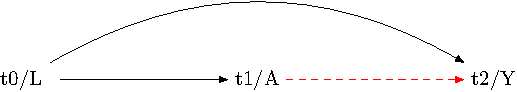
\includegraphics[width=0.8\textwidth,height=\textheight]{causal-tutorial-env_files/figure-pdf/fig-dag-common-cause-1.pdf}

}

\caption{\label{fig-dag-common-cause}Counfounding by a common cause. The
dashed path indicates bias arising from the open backdoor path from A to
Y.}

\end{figure}

\hypertarget{advice-attend-to-the-temporal-order-of-all-measured-variables}{%
\subsubsection{Advice: attend to the temporal order of all measured
variables}\label{advice-attend-to-the-temporal-order-of-all-measured-variables}}

Addressing confounding by a common cause involves its adjustment. This
adjustment effectively closes the backdoor path from the exposure to the
outcome. Equivalently, conditioning on \(L\) d-separates \(A\) and
\(Y\). Common adjustment methods include regression, matching, inverse
probability of treatment weighting, and G-methods (covered in
(\protect\hyperlink{ref-hernuxe1n2023}{Hernán and Monge 2023})).
Figure~\ref{fig-dag-common-cause-solution} clarifies that any confounder
that is a common cause of both \(A\) and \(Y\) must precede \(A\) (and
hence \(Y\)), since effects follow their causes chronologically.

After we have time-indexing the nodes on the graph it becomes evident
that \textbf{control of confounding generally necessitates time-series
data.}

\begin{figure}

{\centering 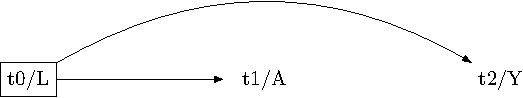
\includegraphics[width=0.8\textwidth,height=\textheight]{causal-tutorial-env_files/figure-pdf/fig-dag-common-cause-solution-1.pdf}

}

\caption{\label{fig-dag-common-cause-solution}Solution: adjust for
pre-exposure confounder. The implication: obtain time series data to
ensure the confounder occurs before the exposure.}

\end{figure}

\hypertarget{confounding-by-collider-stratification-conditioning-on-a-common-effect}{%
\subsubsection{2. Confounding by collider stratification (conditioning
on a common
effect)}\label{confounding-by-collider-stratification-conditioning-on-a-common-effect}}

Conditioning on a common effect, also known as collider stratification,
occurs when a variable, denoted by \(L\), is influenced by both the
exposure, denoted by \(A\), and the outcome, denoted by \(Y\).

Imagine, in the context of green spaces, an individual's choice to live
closer to green spaces (exposure \(A\)) and their improved mental health
(outcome \(Y\)) are both influencing the individual's overall
satisfaction with life (common effect \(L\)). Initially, \(A\) and \(Y\)
could be independent, represented as \(A \coprod Y(a)\), suggesting that
the decision to live near green spaces is not directly causing improved
mental health.

However, when we condition on the life satisfaction \(L\) (the common
effect of \(A\) and \(Y\)), a backdoor path between \(A\) and \(Y\) is
opened. This could potentially induce a non-causal association between
living closer to green spaces and improved mental health. The reason
behind this is that the overall life satisfaction \(L\) can provide
information about both the proximity to green spaces \(A\) and the
mental health status \(Y\). Hence, it may appear that there is an
association between \(A\) and \(Y\) even when there may not be a direct
causal relationship.

\begin{figure}

{\centering 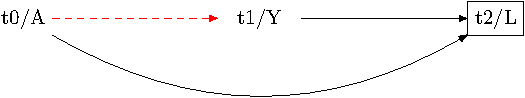
\includegraphics[width=0.8\textwidth,height=\textheight]{causal-tutorial-env_files/figure-pdf/fig-dag-common-effect-1.pdf}

}

\caption{\label{fig-dag-common-effect}Confounding by conditioning on a
collider. The dashed red path indicates bias from the open backdoor path
from A to Y.}

\end{figure}

\hypertarget{advice-attend-to-the-temporal-order-of-all-measured-variables-1}{%
\subsubsection{Advice: attend to the temporal order of all measured
variables}\label{advice-attend-to-the-temporal-order-of-all-measured-variables-1}}

To address the problem of conditioning on a common effect, we should
\emph{generally} ensure that:

\begin{enumerate}
\def\labelenumi{\arabic{enumi}.}
\tightlist
\item
  all confounders \(L\) that are common causes of the exposure \(A\) and
  the outcome \(Y\) are measured before \(A\) has occurred, and
\item
  \(A\) is measured before \(Y\) has occurred.
\end{enumerate}

If such temporal order is preserved, \(L\) cannot be an effect of \(A\),
and thus neither of \(Y\).\footnote{This rule is not absolute. As
  indicated in Figure~\ref{fig-dag-descendent-solution}, it may be
  helpful in certain circumstances to condition on a confounder that
  occurs after the outcome has occurred.}

\begin{figure}

{\centering 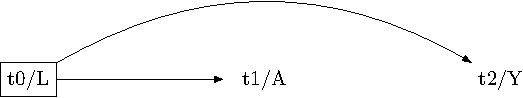
\includegraphics[width=0.8\textwidth,height=\textheight]{causal-tutorial-env_files/figure-pdf/fig-dag-common-effect-solution-1.pdf}

}

\caption{\label{fig-dag-common-effect-solution}Solution: time idexing of
confounders helps to avoid collider bias and maintain d-separation. The
graph makes the imperative clear: we must collect time series data with
confounders measured before the exposure, and that we must likewise
measure the exposure before the outcome, with data collected
repeatitively on the same units.}

\end{figure}

\hypertarget{m-bias-conditioning-on-a-collider-that-occurs-before-the-exposure-may-introduce-bias}{%
\subsubsection{M-bias: conditioning on a collider that occurs before the
exposure may introduce
bias}\label{m-bias-conditioning-on-a-collider-that-occurs-before-the-exposure-may-introduce-bias}}

Typically, indicators for confounders should be included only if they
are known to be measured before their exposures - with notable
exceptions described below in fig-dag-descendent-solution-2.

In the context of green spaces, consider the scenario where an
individual's level of physical activity (\(L\)) is influenced by an
unmeasured factor related to their propensity to live near green spaces
(\(A\)) and another unmeasured factor linked to their mental health
(\(Y\)). Here, physical activity \(L\) does not directly affect the
decision to live near green spaces \(A\) or mental health status \(Y\),
but is a descendent of unmeasured variables that do.

If we condition on physical activity \(L\) in this scenario, we evoke
what is known as ``M-bias''. If \(L\) is neither a common cause of \(A\)
and \(Y\) nor the effect of a shared common cause, then \(L\) should not
be included in a causal model. Figure~\ref{fig-m-bias} represents a case
where \(A \coprod Y(a)\) but \(A \cancel{\coprod} Y(a)| L\).

M-bias is another example of collider stratification bias, a phenomenon
where conditioning on a common effect or a descendent of a common effect
induces an association between variables that were previously
independent (\protect\hyperlink{ref-cole2010}{Cole \emph{et al.}
2010}).\footnote{Note, when we draw a chronologically ordered path from
  left to right the M shape for which ``M-bias'' takes its name changes
  to an E shape We shall avoid proliferating jargon and retain the term
  ``M bias.''}

\begin{figure}

{\centering 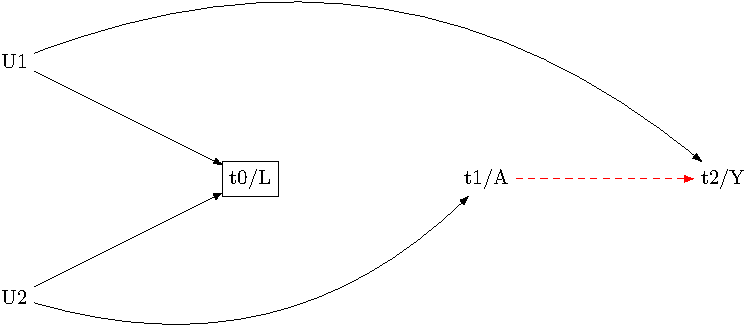
\includegraphics[width=0.8\textwidth,height=\textheight]{causal-tutorial-env_files/figure-pdf/fig-m-bias-1.pdf}

}

\caption{\label{fig-m-bias}M-bias: confounding control by including
previous outcome measures. The dashed red path indicates bias from the
open backdoor path from A to Y by conditioning on pre-exposure variable
L. The solution: do not condition on L. The graph makes it evident that
conditioning on variables measured before the exposure is not sufficient
to prevent confounding.}

\end{figure}

\hypertarget{advice-adopt-the-modified-disjunctive-cause-criterion-for-confounding-control}{%
\subsubsection{Advice: adopt the modified disjunctive cause criterion
for confounding
control}\label{advice-adopt-the-modified-disjunctive-cause-criterion-for-confounding-control}}

Again, the modified disjunctive cause criterion will satisfy the
backdoor criterion in all cases and reduce bias where this criterion
cannot be fully satisfied:

\begin{enumerate}
\def\labelenumi{\alph{enumi}.}
\tightlist
\item
  Control for any variable that causes the exposure, the outcome, or
  both.
\item
  Control for any proxy for an unmeasured variable that is a shared
  cause of both exposure and outcome.
\item
  Define an instrumental variable as a variable associated with the
  exposure but does not influence the outcome independently, except
  through the exposure. Exclude any instrumental variable that is not a
  proxy for an unmeasured confounder from the confounder set (see:
  VanderWeele \emph{et al.}
  (\protect\hyperlink{ref-vanderweele2020}{2020}) page 441,
  (\protect\hyperlink{ref-vanderweele2019}{VanderWeele 2019}))
\end{enumerate}

Of course, the difficulty is in determining which variables belong to a
confounder set. Specialist knowledge can facilitate this task. However,
the data alone typically do not settle this question. (For exceptions
see: bulbulia2021).

\hypertarget{mediator-bias}{%
\subsubsection{3. Mediator bias}\label{mediator-bias}}

Applying this to our green spaces example, again we consider proximity
to green spaces as the exposure (\(A\)), mental health as the outcome
(\(Y\)), and physical activity as the mediator (\(L\)).

In this scenario, living close to green spaces (\(A\)) influences
physical activity (\(L\)), which subsequently impacts mental health
(\(Y\)). If we condition on physical activity (\(L\)), we may bias our
estimates of the total effect of proximity to green spaces (\(A\)) on
mental health (\(Y\)). This bias arises because conditioning on \(L\)
can obscure the direct effect of \(A\) on \(Y\), as it blocks the
indirect path through \(L\). This phenomenon, known as mediator bias, is
depicted in Figure~\ref{fig-dag-mediator}.

One might assume that conditioning on a mediator does not introduce bias
when there is no causal relationship between \(A\) and \(Y\). However,
this is not always the case. Consider a situation where \(L\) is a
common effect of the exposure \(A\) and an unmeasured variable \(U\)
linked to the outcome \(Y\). Here, including \(L\) may inflate the
association between \(A\) and \(Y\), even if \(A\) is not related to
\(Y\) and \(U\) does not cause \(A\). This case is depicted in
Figure~\ref{fig-dag-descendent}.

Hence, unless one is specifically investigating mediation analysis, it
is generally inadvisable to condition on a post-treatment variable.
Being aware of the timeline in the spatial organisation of the graph
underlines a critical principle for data collection: if we cannot
guarantee that \(L\) is measured before \(A\), and if \(A\) may affect
\(L\), including \(L\) in our model could lead to mediator bias. This
scenario is illustrated in Figure~\ref{fig-dag-descendent}.

\begin{figure}

{\centering 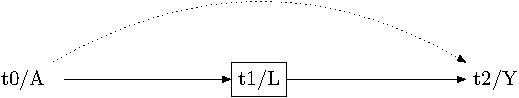
\includegraphics[width=0.8\textwidth,height=\textheight]{causal-tutorial-env_files/figure-pdf/fig-dag-mediator-1.pdf}

}

\caption{\label{fig-dag-mediator}Confounding by conditioning on a
mediator. The dashed black arrow indicates bias arising from partially
blocking the path between A and Y.}

\end{figure}

\hypertarget{advice-attend-to-the-temporal-order-of-all-measured-variables-2}{%
\subsubsection{Advice: attend to the temporal order of all measured
variables}\label{advice-attend-to-the-temporal-order-of-all-measured-variables-2}}

To mitigate the issue of mediator bias, particularly when focusing on
total effects, we should generally avoid conditioning on a mediator. We
avoid this problem by ensuring that \(L\) occurs before the treatment
\(A\) and the outcome \(Y\) (Note: a counter-example is presented in
Figure~\ref{fig-dag-descendent-solution-2}). Again, we discover the
importance of explicitly stating and measuring the temporal order of our
variables.\footnote{Note that if \(L\) were associated with \(Y\) and
  could not be caused by \(A\), conditioning on \(L\) would typically
  enhance the precision of the causal effect estimate of \(A \to Y\).
  This precision enhancement holds even if \(L\) occurs after \(A\).
  However, the onus is on the researcher to show that the post-treatment
  factor cannot be a consequence of the exposure.}

\begin{figure}

{\centering 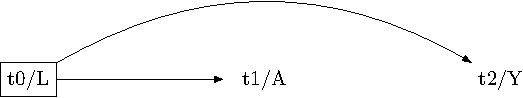
\includegraphics[width=0.8\textwidth,height=\textheight]{causal-tutorial-env_files/figure-pdf/fig-dag-mediator-solution-1.pdf}

}

\caption{\label{fig-dag-mediator-solution}Solution: do not condition on
a mediator. The implication: by ensuring temporal order in data
collection we diminish the probabilty of mistaking an effect of an
exposure for its confounder.}

\end{figure}

\hypertarget{conditioning-on-a-descendant-may-induce-confounding}{%
\subsubsection{4. Conditioning on a descendant may induce
confounding}\label{conditioning-on-a-descendant-may-induce-confounding}}

Let us consider this principle in the context of our green spaces
example. Again denote ``proximity to green spaces'' by \(A\), ``mental
health'' by \(Y\). Denote ``physical activity'' by \(L\), and ``sun
exposure'' by \(L^\prime\).

In this scenario, assume \(L^\prime\), sun exposure, is caused by an
unobserved variable \(U\), and is influenced by \(A\), the proximity to
green spaces. Further, assume \(U\) affects the outcome \(Y\), mental
health.

Conditioning on \(L^\prime\), which is a descendant of \(A\) and \(U\),
can lead to a spurious association between \(A\) and \(Y\) through the
path \(A \to L^\prime \to U \to Y\). This situation, shown in
Figure~\ref{fig-dag-descendent}, illustrates how conditioning on a
descendant can introduce confounding, resulting in a distorted causal
estimation.

\begin{figure}

{\centering 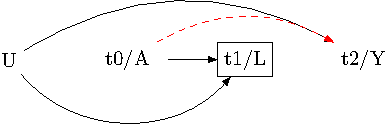
\includegraphics[width=0.8\textwidth,height=\textheight]{causal-tutorial-env_files/figure-pdf/fig-dag-descendent-1.pdf}

}

\caption{\label{fig-dag-descendent}Confounding by descent: the red
dashed path illustrates the introduction of bias by conditioning on the
descendant of a confounder that is affected by the exposure, thus
opening of a backdoor path between the exposure, A, and the outcome, Y.}

\end{figure}

Again, the advice is evident from the chronology of the graph: we should
measure the (\(L^\prime\)) before the exposure (\(A\)). This solution is
presented in Figure~\ref{fig-dag-descendent-solution}.

\begin{figure}

{\centering 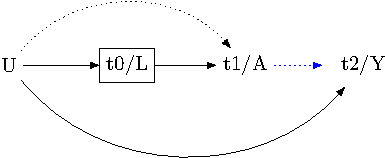
\includegraphics[width=0.8\textwidth,height=\textheight]{causal-tutorial-env_files/figure-pdf/fig-dag-descendent-solution-1.pdf}

}

\caption{\label{fig-dag-descendent-solution}Solution: again the graph
makes it clear that our data must ensure temporal order of the
measurements. By ensuring that L occurs before A confounding is
controlled. The figure also makes it evident that L need not affect Y to
be a confounder (i.e.~a member of a confounder set).}

\end{figure}

\hypertarget{conditioning-on-a-descendent-may-reduce-confounding}{%
\subsubsection{5. Conditioning on a descendent may reduce
confounding}\label{conditioning-on-a-descendent-may-reduce-confounding}}

In our greenspace example, consider an unmeasured confounder \(U\),
perhaps a genetic factor, that impacts both proximity to green spaces
\(A\), mental health \(Y\), and a variable \(L^\prime\), such as a
behavioural trait that only manifests later in life.

As shown in Figure~\ref{fig-dag-descendent-solution-2}, if we adjust for
\(L^\prime\), we might be able to reduce the confounding caused by the
unmeasured \(U\). Even though \(L^\prime\) may occur after the exposure
and even after the outcome, conditioning on it can help control for the
confounding because it acts as a proxy for an unmeasured common cause of
the exposure and the outcome.

This scenario reveals that adhering strictly to a rule that only allows
us to condition on pre-exposure and pre-outcome variables may not always
be optimal. It highlights the need for careful contemplation of data
collection strategies. We cannot resort solely to algorithmic rules for
confounding control. Every case necessitates its unique approach.

\begin{figure}

{\centering 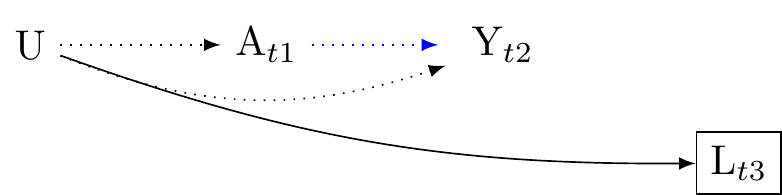
\includegraphics[width=0.8\textwidth,height=\textheight]{causal-tutorial-env_files/figure-pdf/fig-dag-descendent-solution-2-1.pdf}

}

\caption{\label{fig-dag-descendent-solution-2}Solution: conditioning on
a confounder that occurs after the exposure and the outcome might
address a problem of unmeasured confounding if the confounder is a
descendent of a prior common cause of the exposure and outcome. The
dotted paths denote that the effect of U on A and Y is partially
adjusted by conditioning on L', even though L' occurs after the outcome.
The paths are dotted to represent a reduction of bias by conditioning on
the post-outcome descendent of an unmeasured common cause of the
exposure and outcome. How might this work? Consider a genetic factor
that affects the exposure and the outcome early in life might be
measured by an indicator late that is expressed (and may be measured)
later in life. Adjusting for such an indicator would constitute an
example of post-outcome confounding control.}

\end{figure}

\hypertarget{using-causal-diagrams-to-inform-data-collection-the-three-wave-panel-design}{%
\subsubsection{6. Using causal diagrams to inform data collection: the
three-wave panel
design}\label{using-causal-diagrams-to-inform-data-collection-the-three-wave-panel-design}}

In a three-wave panel design, we collect data across three intervals to
facilitate observational causal inference. The causal diagram in
Figure~\ref{fig-dag-6} clarifies the virtues of panel data collection

\begin{enumerate}
\def\labelenumi{\arabic{enumi}.}
\item
  \textbf{Baseline Data Collection}:

  \begin{itemize}
  \item
    \textbf{Confounding Data}: At baseline, we collect data on
    confounders, along with data on the exposure and the outcome. This
    initial data collection phase is crucial for measuring common causes
    of the treatment and outcome, or the descendents of such common
    causes.
  \item
    \textbf{Exposure and Outcome Data}: Baseline measurements of
    exposure and outcome allow our data collection to more effectively
    mimic an experiment.

    \begin{itemize}
    \item
      \textbf{Incidence Effect Evaluation}: The baseline exposure allows
      us to interpret the post-baseline exposure effect as an incidence
      effect rather than a prevalence effect. This interpretation means
      we can assess the change due to a new occurrence (incidence) of
      the exposure rather than its overall presence (prevalence).
    \item
      \textbf{Sample Adequacy for Rare Exposures}: Especially when the
      exposure is uncommon, measuring the baseline exposure and outcome
      can help assess the adequacy of the sample size.
    \item
      \textbf{Temporal Ordering and Confounding Control}: Incorporating
      the outcome at baseline helps confirm the temporal order of the
      cause-effect relationship, thereby guarding against reverse
      causation. Moreover, when we also control for the exposure at
      baseline, an unmeasured confounder would have to negate the
      association between the exposure at one wave post-baseline and the
      outcome at two waves post-baseline, independent of the baseline
      effect.
    \end{itemize}
  \end{itemize}
\item
  \textbf{First Follow-Up Data Collection (Baseline +1)}:

  \begin{itemize}
  \tightlist
  \item
    At this stage, we measure the exposure. This follow-up allows us to
    capture the causal effect of changes in the exposure since baseline.
  \end{itemize}
\item
  \textbf{Second Follow-Up Data Collection (Baseline +2)}:

  \begin{itemize}
  \tightlist
  \item
    We measure the outcome at this stage. Similar to the first
    follow-up, this measurement allows us to capture a controlled effect
    for the outcome since the baseline measurement.
  \end{itemize}
\end{enumerate}

Through this design, any unmeasured confounder affecting both the
exposure and the outcome would need to do so independently of these
baseline measurements of exposure and outcome. Causal diagrams
effectively illustrate this methodology, as shown in
Figure~\ref{fig-dag-6}, clarifying the paths of causation, potential
sources of confounding, and the methods used for controlling these
confounders. As a result, these diagrams are powerful tools for
observational causal inference in a three-wave panel design.

\begin{figure}

{\centering 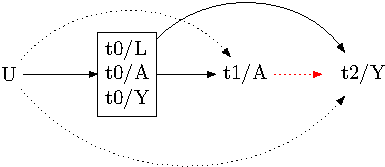
\includegraphics[width=0.8\textwidth,height=\textheight]{causal-tutorial-env_files/figure-pdf/fig-dag-6-1.pdf}

}

\caption{\label{fig-dag-6}Causal diagram adapted from Vanderweele et
al.'s three-wave panel design. The dotted line indicates a reduction in
bias arising from including baseline measures for the exposure and
outcome. For an unmeasured confounder U to bias the exposure-outcome
association, it would need to do so independently of these outcome and
exposure baseline measures. The graph clarifies that by measuring
confounders before the exposure and the exposure before the outcome, we
reduce the potential for reverse causation, collider stratification, and
mediator biases.}

\end{figure}

\hypertarget{the-inevitability-of-unmeasured-confounding}{%
\subsubsection{7. The Inevitability of Unmeasured
Confounding}\label{the-inevitability-of-unmeasured-confounding}}

In observational research, there is an unavoidable issue known as
unmeasured confounding. These are confounders that are not included in
the data set, thus not accounted for during analysis, which can
introduce bias into the study. This may occur due to constraints such as
data availability, financial or ethical reasons. Despite all efforts, it
is virtually impossible to measure and control for every possible
confounder. Therefore, it is necessary to estimate the potential impact
of these unmeasured confounders and consider their influence on the
study's findings.

One of the methods to assess the potential impact of unmeasured
confounding is through sensitivity analysis, which quantifies how strong
an unmeasured confounder would need to be to fully explain away an
observed association. A commonly used metric for this purpose is the
E-Value.

The E-Value quantifies the minimum strength of association that an
unmeasured confounder would require with both the exposure and outcome,
over and above the measured confounders, to explain away an observed
exposure-outcome association. An E-Value close to 1 suggests that the
observed association is vulnerable to unmeasured confounding, whereas a
high E-Value suggests that a remarkably strong unmeasured confounder
would be necessary to explain the observed association, thus providing
evidence towards the robustness of the observed association.

E-Values can be computed through the \texttt{EValue} package in R
(\protect\hyperlink{ref-mathur2018}{Mathur \emph{et al.} 2018}). This
package provides an intuitive, user-friendly interface for researchers
to compute E-Values. Observational researchers have no excuses not to
conduct sensitivity analyses.

\hypertarget{part-3.-summary-pitfalls-and-tips.}{%
\subsubsection{Part 3. Summary, Pitfalls and
Tips.}\label{part-3.-summary-pitfalls-and-tips.}}

\hypertarget{summary}{%
\subsubsection{Summary}\label{summary}}

We introduced the potential outcomes framework of causal inference,
focussing on three fundamental assumptions:

\begin{enumerate}
\def\labelenumi{\arabic{enumi}.}
\item
  \textbf{Causal Consistency}: This assumption posits that for every
  unit, the outcome under treatment is equal to the observed outcome if
  the unit was treated, and vice versa for non-treatment. In essence, it
  says that `the treatment' is consistently defined.
\item
  \textbf{Exchangeability}: The assignment of treatment is random and
  independent of the potential outcomes. This is a essential virtue of
  experimental designs The process of randomisation ensures that every
  participant has an equal chance of being assigned to the treatment or
  control group, creating balance in the factors that might affect the
  outcomes under the different treatments. Randomisation is powerful
  because it removes any systematic bias in the treatment assignment.
\item
  \textbf{Positivity}: Each unit under study has a non-zero probability
  of receiving the treatment. This ensures that comparisons between
  treated and untreated units are meaningful and well-defined.
\end{enumerate}

We observed that in the context of randomised experiments, these
assumptions are generally met, and in being met, experimentalists
address the problem of missing potential outcomes in the treatment
groups that researchers compare.

Having built core intuitions for how experiments recover average causal
effect estimates, we considered how the three fundamental assumptions
required for causal inferences may be easily violated in observational
studies. Where treatment assignment is not random and can be influenced
by observed or unobserved variables, correlation is not equivalent to
causation.

Next, we clarified the conditions where, assuming the three fundamental
assumptions of causal inference have been satisified, we may to recover
causal effect estimates from observational data.

To obtain such causal effect estimates we must:

\begin{itemize}
\tightlist
\item
  Precisely defining the interventions that need to be compared.
\item
  Conditioning on confounders, variables associated with both the
  treatment and the outcome, or that are descendents of such common
  causes.
\item
  Ensuring positivity, that is, each individual has some probability of
  receiving each level of treatment. This ensures the comparability of
  treatment groups.
\end{itemize}

The second part of the article discusses the use of causal diagrams for
dealing with identification problems in observational settings. The key
points take home messages were:

\begin{itemize}
\tightlist
\item
  For confounding control to work, researchers generally require
  time-series data that determine the temporal order of events.
\item
  Causal diagrams reveal that the three-wave panel design is a powerful
  tool for addressing causal questions with observational data.
\item
  Nevertheless, sensitivity analysis should always be performed, and can
  be performed relatively easily.
\end{itemize}

We conclude by summarising our advice through ``Tips'' and ``Pitfalls''

\hypertarget{data-collection-tips}{%
\subsubsection{Data Collection Tips}\label{data-collection-tips}}

\begin{enumerate}
\def\labelenumi{\arabic{enumi}.}
\tightlist
\item
  Use time series data.
\item
  Ensure significant change from baseline in treatment (positivity).
\item
  Clearly define measurements for treatment, outcome, and baseline
  confounders.
\item
  Include baseline treatment measures.
\item
  Include baseline outcome measures.
\item
  Strive for high sample retention.
\end{enumerate}

\hypertarget{graph-drawing-tips}{%
\subsubsection{Graph Drawing Tips}\label{graph-drawing-tips}}

\begin{enumerate}
\def\labelenumi{\arabic{enumi}.}
\tightlist
\item
  Define all nodes unambiguously.
\item
  Keep the graph simple and focused.
\item
  Explicitly state any novel conventions.
\item
  Maintain acyclicity in the graph.
\item
  Arrange nodes in chronological order.
\item
  Time-stamp nodes to reflect the temporal sequence of causation.
\item
  Apply a modified disjunctive cause criterion pragmatically.
\item
  Add nodes for unmeasured confounding where helpful.
\item
  Illustrate nodes for post-treatment selection.
\item
  Remember, causal diagrams are qualitative tools, not detailed maps.
\end{enumerate}

\hypertarget{pitfalls-to-avoid}{%
\subsubsection{Pitfalls to Avoid}\label{pitfalls-to-avoid}}

\begin{enumerate}
\def\labelenumi{\arabic{enumi}.}
\tightlist
\item
  Avoid using cross-sectional data.
\item
  Don't misuse causal diagrams without understanding counter-factual
  data science.
\item
  Don't create diagrams without time indices.
\item
  Avoid excessive nodes in the graph.
\item
  Don't draw arrows into the manipulation in experimental studies.
\item
  Don't inaccurately describe bias when exposure and outcome are
  d-separated.
\item
  Don't ignore causal diagrams during research design.
\item
  Avoid representing interactions and non-linear dynamics in causal
  diagrams.
\item
  Remember that structural equation models are not true structural
  models: do not mistake structural equation models for causal diagrams
  (NOTE Don, we haven't yet said this, but we should!)
\end{enumerate}

\newpage{}

\hypertarget{funding}{%
\subsection{Funding}\label{funding}}

This work is supported by a grant from the Templeton Religion Trust
(TRT0418). JB received support from the Max Planck Institute for the
Science of Human History. The funders had no role in preparing the
manuscript or the decision to publish it.

\hypertarget{references}{%
\subsection{References}\label{references}}

\hypertarget{refs}{}
\begin{CSLReferences}{1}{0}
\leavevmode\vadjust pre{\hypertarget{ref-bulbulia2022}{}}%
Bulbulia, JA (2022) A workflow for causal inference in cross-cultural
psychology. \emph{Religion, Brain \& Behavior}, \textbf{0}(0), 1--16.
doi:\href{https://doi.org/10.1080/2153599X.2022.2070245}{10.1080/2153599X.2022.2070245}.

\leavevmode\vadjust pre{\hypertarget{ref-cole2010}{}}%
Cole, SR, Platt, RW, Schisterman, EF, \ldots{} Poole, C (2010)
Illustrating bias due to conditioning on a collider. \emph{International
Journal of Epidemiology}, \textbf{39}(2), 417--420.
doi:\href{https://doi.org/10.1093/ije/dyp334}{10.1093/ije/dyp334}.

\leavevmode\vadjust pre{\hypertarget{ref-edwards2015}{}}%
Edwards, JK, Cole, SR, and Westreich, D (2015) All your data are always
missing: Incorporating bias due to measurement error into the potential
outcomes framework. \emph{International Journal of Epidemiology},
\textbf{44}(4), 14521459.

\leavevmode\vadjust pre{\hypertarget{ref-greenland1999}{}}%
Greenland, S, Pearl, J, and Robins, JM (1999) Causal diagrams for
epidemiologic research. \emph{Epidemiology (Cambridge, Mass.)},
\textbf{10}(1), 37--48.

\leavevmode\vadjust pre{\hypertarget{ref-hernan2023}{}}%
Hernan, MA, and Robins, JM (2023) \emph{Causal inference}, Taylor \&
Francis. Retrieved from
\url{https://books.google.co.nz/books?id=/_KnHIAAACAAJ}

\leavevmode\vadjust pre{\hypertarget{ref-hernuxe1n2023}{}}%
Hernán, MA, and Monge, S (2023) Selection bias due to conditioning on a
collider. \emph{BMJ}, \textbf{381}, p1135.
doi:\href{https://doi.org/10.1136/bmj.p1135}{10.1136/bmj.p1135}.

\leavevmode\vadjust pre{\hypertarget{ref-holland1986}{}}%
Holland, PW (1986) Statistics and causal inference. \emph{Journal of the
American Statistical Association}, \textbf{81}(396), 945960.

\leavevmode\vadjust pre{\hypertarget{ref-mathur2018}{}}%
Mathur, MB, Ding, P, Riddell, CA, and VanderWeele, TJ (2018) Website and
r package for computing e-values. \emph{Epidemiology (Cambridge,
Mass.)}, \textbf{29}(5), e45.

\leavevmode\vadjust pre{\hypertarget{ref-mcelreath2020}{}}%
McElreath, R (2020) \emph{Statistical rethinking: A bayesian course with
examples in r and stan}, CRC press.

\leavevmode\vadjust pre{\hypertarget{ref-pearl2009}{}}%
Pearl, J (2009) \emph{\href{https://doi.org/10.1214/09-SS057}{Causal
inference in statistics: An overview}}.

\leavevmode\vadjust pre{\hypertarget{ref-pearl1995}{}}%
Pearl, J, and Robins, JM (1995) Probabilistic evaluation of sequential
plans from causal models with hidden variables. In, Vol. 95, Citeseer,
444453.

\leavevmode\vadjust pre{\hypertarget{ref-rohrer2018}{}}%
Rohrer, JM (2018) Thinking clearly about correlations and causation:
Graphical causal models for observational data. \emph{Advances in
Methods and Practices in Psychological Science}, \textbf{1}(1), 2742.

\leavevmode\vadjust pre{\hypertarget{ref-rubin1976}{}}%
Rubin, DB (1976) Inference and missing data. \emph{Biometrika},
\textbf{63}(3), 581--592.
doi:\href{https://doi.org/10.1093/biomet/63.3.581}{10.1093/biomet/63.3.581}.

\leavevmode\vadjust pre{\hypertarget{ref-vanderweele2015}{}}%
VanderWeele, T (2015) \emph{Explanation in causal inference: Methods for
mediation and interaction}, Oxford University Press.

\leavevmode\vadjust pre{\hypertarget{ref-vanderweele2009}{}}%
VanderWeele, TJ (2009) Concerning the consistency assumption in causal
inference. \emph{Epidemiology}, \textbf{20}(6), 880.
doi:\href{https://doi.org/10.1097/EDE.0b013e3181bd5638}{10.1097/EDE.0b013e3181bd5638}.

\leavevmode\vadjust pre{\hypertarget{ref-vanderweele2018}{}}%
VanderWeele, TJ (2018) On well-defined hypothetical interventions in the
potential outcomes framework. \emph{Epidemiology}, \textbf{29}(4), e24.
doi:\href{https://doi.org/10.1097/EDE.0000000000000823}{10.1097/EDE.0000000000000823}.

\leavevmode\vadjust pre{\hypertarget{ref-vanderweele2019}{}}%
VanderWeele, TJ (2019) Principles of confounder selection.
\emph{European Journal of Epidemiology}, \textbf{34}(3), 211219.

\leavevmode\vadjust pre{\hypertarget{ref-vanderweele2013}{}}%
VanderWeele, TJ, and Hernan, MA (2013) Causal inference under multiple
versions of treatment. \emph{Journal of Causal Inference},
\textbf{1}(1), 120.

\leavevmode\vadjust pre{\hypertarget{ref-vanderweele2020}{}}%
VanderWeele, TJ, Mathur, MB, and Chen, Y (2020) Outcome-wide
longitudinal designs for causal inference: A new template for empirical
studies. \emph{Statistical Science}, \textbf{35}(3), 437466.

\leavevmode\vadjust pre{\hypertarget{ref-westreich2010}{}}%
Westreich, D, and Cole, SR (2010) Invited commentary: positivity in
practice. \emph{American Journal of Epidemiology}, \textbf{171}(6).
doi:\href{https://doi.org/10.1093/aje/kwp436}{10.1093/aje/kwp436}.

\leavevmode\vadjust pre{\hypertarget{ref-westreich2015}{}}%
Westreich, D, Edwards, JK, Cole, SR, Platt, RW, Mumford, SL, and
Schisterman, EF (2015) Imputation approaches for potential outcomes in
causal inference. \emph{International Journal of Epidemiology},
\textbf{44}(5), 17311737.

\end{CSLReferences}



\end{document}
